\documentclass[10pt,journal,compsoc,twoside]{IEEEtran}

\usepackage[OT1]{fontenc} 
\usepackage{epsfig}
\usepackage{graphicx}
\usepackage{amsmath}
\usepackage{amssymb}
\usepackage[backref=true]{biblatex}
\usepackage{hyperref}
\usepackage{listings}
\usepackage{algorithm}
\usepackage[noend]{algpseudocode}
\usepackage{stfloats}
\usepackage{algorithm}
\usepackage[noend]{algpseudocode}
\usepackage{subcaption}
\usepackage{amsthm}
\usepackage{tabu}

\newcommand{\etal}{\textit{et al}. }
\newcommand{\ie}{\textit{i}.\textit{e}., }
\newcommand{\eg}{\textit{e}.\textit{g}. }
\newcommand{\Lagr}{\mathcal{L}}

\newtheorem{theorem}{Theorem}

\addbibresource{bibliography.bib}

\begin{document}
	
	\title{Video Retrieval Using Self-Supervised Deep Representations}
	
	\author{Max Ehrlich, Peng Zhao, Xiawu Sun, Bhargavi Patel}
	
	\markboth{CS828J}{University of Maryland}
	
	\IEEEtitleabstractindextext{%
		\begin{abstract}
			 In the video retrieval problem, we seek to find, in an automated way, videos that have similar semantic or visual properties. Traditional techniques project videos into a high dimensional space using feature extraction and finding nearest-neighbors in the feature space. Recent work has focused on using deep neural-networks to learn the feature space, which requires a large dataset of labeled data. We propose a novel method for generating video retrieval representations based on self-supversied deep networks. Our method combines two self-supervised representations, Odd-One-Out (O3N), and Temporal Smoothness, which allows the network to learn without labeled data. We show that combining the O3N loss and the Temporal Smoothness loss leads to increased accuracy over using the O3N loss alone. We further provide qualitative results for the retrieval properties of our represntation using both simple k nearest neighbors search and hamming similarity from locality sensitive hashes.
		\end{abstract}
	}
	
	\maketitle
	
	\IEEEdisplaynontitleabstractindextext
	
	\IEEEpeerreviewmaketitle
	
	\IEEEraisesectionheading{\section{Introduction}\label{sec:intro}}
	
\IEEEPARstart{T}{he} goal of the video retrieval problem is to locate videos in a database satisfying a given set of criteria. This is a well studied problem in the field of visual information retrieval (TODO CITATIONS). In general, there are two major criteria that are used to locate videos: visual similarity and semantic similarity. Formally, given a set of videos $V = \{v_0, ..., v_N\}$ and a probe video $p$, the visual similarity criterion seeks to return a sequence $S_v$ of elements from $V$ such that, given some visual similarity function $\sigma_{\text{visual}}(x, y)$

\begin{equation*}
    S_v = (v_i, v_k, ..., v_j)
\end{equation*}
such that 

\begin{equation*}
\sigma_{\text{visual}}(p, v_i) > \sigma_{\text{visual}}(p, v_k) > ... > \sigma_{\text{visual}}(p, v_j)
\end{equation*}
The principal task being to develop $\sigma_{\text{visual}}(x, y)$ such that the majority of human observers agree on the sequence $S_v$. For example, this kind of retrieval system might find all pictures with blue backgrounds, or all videos with high motion blur, depending on the probe $p$. 

The semantic similarity criterion can be phrased in two distinct ways. The first, similar to the visual similarity criterion, given $V$, $p$, and a semantic similarity function $\sigma_{\text{semantic}}(x, y)$, the sequence $S_s$ is generated such that $\sigma_{\text{semantic}}(p, v_i) > ... > \sigma_{\text{semantic}}(p, v_j)$. Again the goal here is to agree with human observers. An alternative, and interesting, formulation of the semantic criterion is to associate a set of text labels with the videos in $V$. Then instead of a probe video $p$, a set of probe labels of arbitrary cardinality is provided and videos containing those text labels are returned as in traditional database management systems. The task now is how to analyze the videos in $V$ and produce the text labels, or, how to match videos given text labels not seen before akin to zero-shot learning. While this provides a general overview of the type of tasks usually associated with the video retrieval problem, we focus on the cases where a probe video is given.

Using the expressive power of deep neural-networks, which have revolutionized the field of computer vision since their resurgence on 2012, we propose a novel similarity function that can learn, in a self-supervised way, similarity \textit{both} visually and in semantics. Our network combines two loss functions, the Odd-One-Out loss and the Temporal Smoothness loss (TODO cite these). Additionally, we redesign the network architecture to take advantage of these loss functions. Videos are then projected into the \textit{embedding space} defined by the network, and we define the similarity measure of two videos as 

\begin{equation*}
\sigma(x, y) =|f(x) - f(y)|_2
\end{equation*}
where $f(x)$ uses the learned network to project videos into the embedding space and $|\cdot|_2$ denotes the $l_2$ norm. 

Since the space defined by our network is high dimensional, we additionally test a well studied optimization to the search problem, locality sensitive hashing (LSH). LSH defines a hash function $H(x)$ such that, in general, the relative distance between points in space is preserved after hashing. Formally, given three points in some space $x_0, x_1, x_2$ such that 

\begin{equation*}
|x_0 - x_1|_2 > |x_0 - x_2|_2
\end{equation*}
then

\begin{equation*}
|H(x_0) - H(x_1)|_2 > |H(x_0) - H(x_2)|_2
\end{equation*}

We choose the Random Projections algorithm for our hash function. The Random Projections algorithm takes $N$ random hyperplanes in the space of the original points and encodes with a single bit, the side of the hyperplane a given point resides on. This results in an $N$ bit signature for each point. Points can then be compared using the Hamming distance, which can be computed quickly. We are free to vary the number of bits with a corresponding change in the accuracy of the result.

    
    \section{Related Work}\label{sec:related}
Vast amount of video stored in web archives makes their retrieval based on manual text annotations impractical.
Unsupervised methods provide an edge for videos in terms of action classification, detection and retrieval as manual annotations is not required. 
For retrieval of videos in an unsupervised method we need to exploit the data to find similar semantic and visual properties.

Most of the traditional techniques uses hand crafted features such as Histogram of Oriented Gradients (HOG),Histogram of Optical Flow (HOF), Motion Boundary Histogram
(MBH) around spatio-temporal interest points \cite{Laptev08learningrealistic} or in dense grid to learn features or around dense point trajectories obtained through optical flow based tracking to learn the feature vectors. 

For video retrieval and self supervised learning of the features the direction of time-flow (forward or backward) in videos was studied \cite{Pickupetal14}. CNNs are used to explore the power of learning
slow features, also referred to as “temporally coherent” features\cite{Mobahi2009}
The approach\cite{podlesnaya2016retrieval} does video indexing and retrieval using convulational neural network  based on unified semantic features.

CNN-based unsupervised representation learning method \cite{Misra2016ShuffleAL}where the learning task is to verify whether a sequence
of frames from a video is presented in the correct order or
not.The method does not learn to encode temporal
information but only spatial. In contrast \cite{fernando2017self}
exploits the analogical reasoning over sequences and pose
the feature learning problem as a  $ N + 1 $ way multi class
classification problem which is much harder than the binary
verification problem. In this paper the methods specified in odd-one-out \cite{fernando2017self} with temporal smoothness is combines to learn features for video retrieval.
    
    \section{Odd One Out Learning}

Odd-one-out uses temporal ordering for representation learning in self supervised way.
This networks is a new way to learn visual features for videos without using category level annotations.This method is applied to self supervised video representation learning where they sample sub sequences from videos and ask the network to learn to predict the odd video sequence.Here the odd video sub sequence is sampled such that it has wrong temporal order of frames while the even ones have the correct temporal order. 
They transfer weights to action recognition and fine tune on supervised set and show improvement over fully supervised learning.

Given $(N+1)$ number of sub sequenced videos from one single video, N are in correct chronological order of frames which is the even set. The odd set consist of frame sampled from invalid sub sequenced video. One out of $(N+1)$ element is odd object.

Further more the position of the odd element is randomized by shuffling sequence permutation.
Thus the odd one out prediction task reduces to an $(N+1)$ way classification problem, which can be solved by maximum likelihood estimation. 

The Model :  Multi Branch Convolutional neural Network consist of $(N+1)$ input branches. 
Each contain 5 Convolutional layers. 
The fusion layer -- merges the information from $(N+1)$ branches after the first fully connected layer. And helps to find regularities and pick the element with irregularities. 
Two models are : 
1. Concatenation Model 
2. Sum of difference. 

    
    \section{Temporal Smoothness}

Besides the odd-one-out question, temporal smoothness can be exploited to learn high-level concepts from unlabeled video.
This is motivated by dimensionality reduction, which aims to translate high dimensional data to a low dimensional representation such that similar input objects are mapped to nearby points in feature space. 
In this this section, we first provide a brief review of a temporal smoothness prior work that is first used in a dimensionality reduction algorithm called Dimensionality Reduction by Learning an Invariant Mapping (DrLIM). Then we present several improvements on the prior work and fit it in our problem. 

Consider a set of input vectors $I = \{x_1, ..., x_p\}$ and a parametric function $G_W$ returns extracted features. 
For each $x_i \in I$ there exist a subset of vectors in $I$ that are deemed as similar to $x_i$.  
Let $x_1, x_2 \in I$ be a pair of input vectors and $Y$ be a binary label assigned to this pair.
$Y = 0$ if $x_1$ and $x_2$ are deemed similar, and $Y = 1$ if they are deemed dissimilar.
Define the parameterized distance function to be learned $D_W$ between $x_1, x_2$ as the euclidean distance between the outputs of $G_W$ . 
That is,
\begin{equation}
    D_W(x_1, x_2) = || G_W(x_1) - G_W(x_2)||_2
\end{equation}
To shorten notation, $D_W (x_1, x_2)$ is written as $D_W$ . Then the proposed loss function is
\begin{align}
\lagr(W) = \sum_i \lagr(W, (Y, x_1, x_2)^i) \\
\lagr(W, (Y, x_1, x_2)^i) = (1-Y) \lagr_S (D_W^i) + Y \lagr_D (D_W^i)
\end{align}
where $(Y, x_1, x_2)^i$ is the $i$-th labeled sample pair, $\lagr_S$ is the partial loss function for a pair of similar points, $\lagr_D$ the partial loss function for a pair of dissimilar points. 

$\lagr_S$ and $\lagr_D$ must be designed such that minimizing $\lagr$ with respect to $W$ would result in low values of $D_W$ for similar pairs and high values of $D_W$ for dissimilar pairs. In specific, they can be designed as following 
\begin{align}
\lagr_S (D_W^i) = \frac{1}{2} (D_W)^2
\lagr_D (D_W^i) = \frac{1}{2} (max\{0, m - D_W\})^2
\end{align}
Figure~\ref{fig:twoloss} shows these two loss functions. Then the total loss function is 
\begin{equation}
\lagr(W, Y, x_1, x_2) = (1-Y) \frac{1}{2} (D_W)^2 + (Y) \frac{1}{2} (max\{0, m - D_W\})^2
\end{equation}

\begin{figure}
\centering
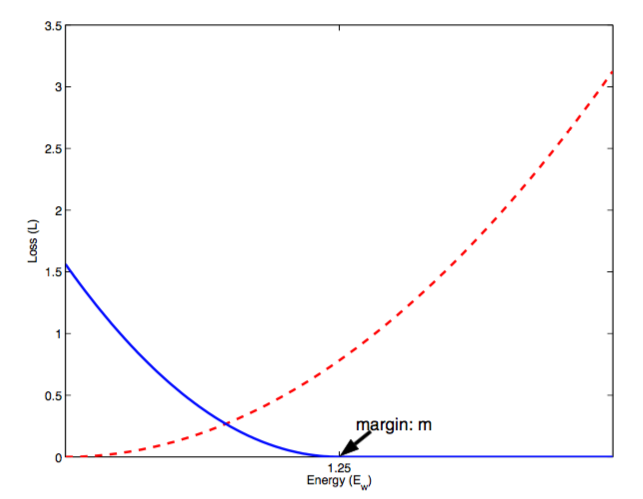
\includegraphics[width=0.5\textwidth]{images/twoloss.png}
\caption{Graph of the loss function $L$ against the energy $D_W$. The dashed (red) line is the loss function for the similar pairs and the solid (blue) line is for the dissimilar pairs.}
\label{fig:twoloss}
\end{figure}

This loss formalization can be directly implemented in temporal coherence. Consider $x_t$ and $x_t\rq{}$ are input frames at two different times, then smoothness loss for a single sample pair can be written as:
\begin{equation}
\begin{split}
\lagr_T(x_t, x_t, W) = \\
     \begin{cases}
        ||G_W(x_t) - G_W(x_t\rq{})||_p & \text{if} |t-t\rq{}| = 1\\
        max(0, m - ||G_W(x_t) - G_W(x_t\rq{})||_p) &\text{if} |t-t\rq{}| > 1 \\
    \end{cases}
\end{split}
\end{equation}

The margin $m$ is introduced to avoid the degenerate solution $G_W(x_t) = G_W(x_0)$ for all $t$. 
Specifically, this margin term encourages data samples that are not temporal neighbors to be separated by at least a distance of $m$-units in feature space. 

However, the second contrastive term in loss $\lagr_T(x_t, x_t\rq{}, W)$ only depends on pairwise distances in the feature space, and hence does not guarantee that the resulting feature space is informative with respect to the input. 
One improvement is to replace this contrastive term with a term that penalizes the reconstruction error of both data samples. 
This reconstruction term not only prevents the constant solution but also acts to explicitly preserve information about the input.

Another improvement is to extract temporal slow features by applying pooling operators in feature space. 
In natural video and on small spatial scales these features mainly correspond to local translations and deformations. 
Invariances to such changes can be achieved using appropriate pooling operators.
We divide each feature vector into $K$ potentially overlapping neighborhoods and denote each of them as $P_i$. 
Specifically, we apply $l_2$-Pooling and the loss discussed above can be expressed as following:
\begin{equation}
\begin{split}
\lagr_T(x_t, x_t\rq{}, W) = \sum_{\tau = \{t, t\rq{}\}} (||W_d G_W(x_\tau) - x_\tau||^2 + \alpha |G_W(x_\tau)|) \\
+ \beta \sum_{i=1}^K |||G_W(t)||^{P_i} -  ||G_W(t\rq{})||^{P_i}|
\end{split}
\end{equation}

    
    \section{Network}\label{sec:network}

Our network architecture contains two copies of the odd-one-out network in order to learn both temporal order and smoothness at the same time. 
The input frames are sampled from sequenced videos with $N+1$ input clips for each odd-one-out network.
As mentioned in the previous section, only one out of the $N+1$ clips is out of order. 
Furthermore, two clips that are chronologically close in the same video are used to feed the two copies of odd-one-out network. 
Figure~\ref{fig:network} is a demonstration with $N=1$.
In particular, clips from the same sequence of video, such as $c_0$ and $c_0\rq{}$, are inputs for the two odd-one-out networks seperately.  
For each odd-one-out network, only one clip is out of order, such as either $c_0$ or $c_1$ for the \lq\lq{}left\rq\rq{} network.

This network architecture makes it possible to consider out-of-order loss $\lagr_{O3N}$ and temporal smoothness loss $\lagr_T$ at the same time. 
Both losses have been discussed in previous sections, and can be combined as loss for the proposed network:
\begin{equation}
\lagr = \lagr_{O3N} + \gamma \lagr_T    
\end{equation}

where hyperparameter $\gamma$ captures the priority between the two losses. 
This paper is the first attempt to combine odd-one-out learning with temporal cohence, and a non-trivial choice of $\gamma$ provides insights to the effectiveness of this learning strategy.

\begin{figure}
\centering
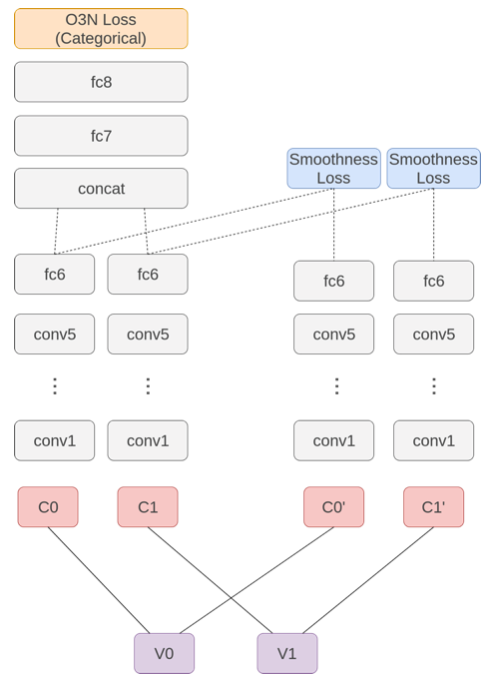
\includegraphics[width=0.35\textwidth]{images/network.png}
\caption{Network architecture.}
\label{fig:network}
\end{figure}
    
    \section{Locality Sensitive Hashing}\label{sec:hashing}

The embedding defined by our joint network architecture is a high dimensional space. Taking the last fully-connected layer of the tuple branches to be the embedding for a tuple gives a point in a 128 dimensional space. The naive retrieval algorithm would then project all videos in the database into this space, then for each probe, project it into the same space and execute a nearest neighbor search. The search would return video ranked by their $l_2$ distance in the 128 dimensional space.

Generally, this is a slow computation. Note that for a single comparison, 

\begin{equation}
    d(x, y) = \sqrt{\sum_{i=0}^{128} (x_i - y_i)^2}
\end{equation} 
Being optimistic and ignoring the square root, this requires 256 additions and 128 multiplies per video in the database, after which $N$ comparisons must be made for a database of size $N$. This does not scale well to large databases.

There are several potential solutions to this which all amount to a dimensionality reduction. We choose a highly efficient method: Locality Sensitive Hashing (LSH). Most hash functions, such as those used in cryptography or for $O(1)$ storage mechanisms, try to distribute their results evenly in the output space. For example, a cryptographically secure hash should result in a distribution of the output bits that appears random to an observer with no knowledge of the input. For a LSH, the goal is the opposite. Inputs should preserve the ordering of their distances when projected into the hashed space. Formally, given three points in some space $x_0, x_1, x_2$ such that 

\begin{equation}
|x_0 - x_1|_2 > |x_0 - x_2|_2
\end{equation}
we desire

\begin{equation}
d(H(x_0), H(x_1)) > d(H(x_0) - H(x_2))
\end{equation}
for some distance function $d()$ defined suitably in the hash space.

We choose the Random Projections, or SimHash \cite{charikar2002similarity}, algorithm for this purpose. The Random Projections algorithm defines $k$ random hyperplanes in the space of the original points. For each point $x$, the hash function $H(x)$ computes

\begin{align}
    p_i = \text{sign}(k_i \cdot x) \\
    H(x) = p_0...p_k
\end{align}

Such that each of the $p_i$ are encoded as a single bit. In this way, the function $H(x)$ defines a $k$-bit Hamming space \cite{hamming1950error}. The $k$ hyperplanes should be uniformly distributed in the input space. Using this algorithm allows us to use the Hamming distance function, which is extremely fast to compute using bitwise operations \cite{cohen1997covering}.

\begin{figure}[h]
    \centering
    \begin{subfigure}[t]{0.24\textwidth}
            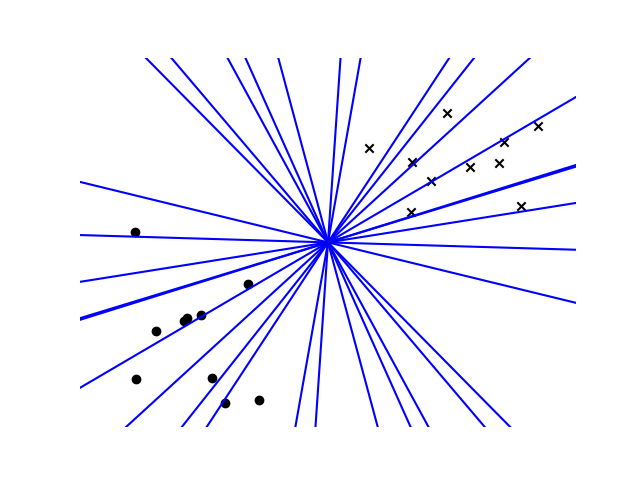
\includegraphics[width=\textwidth]{images/lsh_planes.png}
            \caption{Hyperplanes and points in 2D space.}   
            \label{fig:lshplanes}   
    \end{subfigure} 
    \begin{subfigure}[t]{0.24\textwidth}
            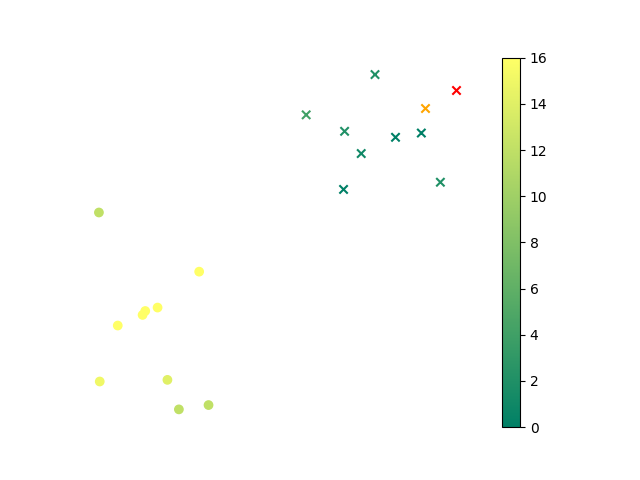
\includegraphics[width=\textwidth]{images/lsh_distance.png}
            \caption{Hamming distance from red point to all other points. Nearest neighbor in hamming space is highlighted in orange.}
            \label{fig:lshdist}
    \end{subfigure}
    \caption{Illustration of the Random Projections algorithm.}
    \label{fig:lsh}
\end{figure}

The number of hyperplanes $k$ is a tunable parameter. In general, a higher $k$ gives more accurate distances for a slower distance computation. Figure \ref{fig:lshplanes} shows a set of 16 hyperplanes that could be used to encode the set of 2D points. Figure \ref{fig:lshdist} ranks the points based on their distance from the red point, with the nearest neighbor in hamming space highlighted in orange. Examining Figure \ref{fig:lshplanes} gives some intuition about why the Random Projections algorithm works: as the number of planes goes to infinity, the distance metric approaches the cosine distance between the points. This intuitive result is proven by Charikar \cite{charikar2002similarity}.


    
    \section{Results}\label{sec:results}

\begin{figure}[t]
    \centering
    \begin{subfigure}[t]{0.24\textwidth}
        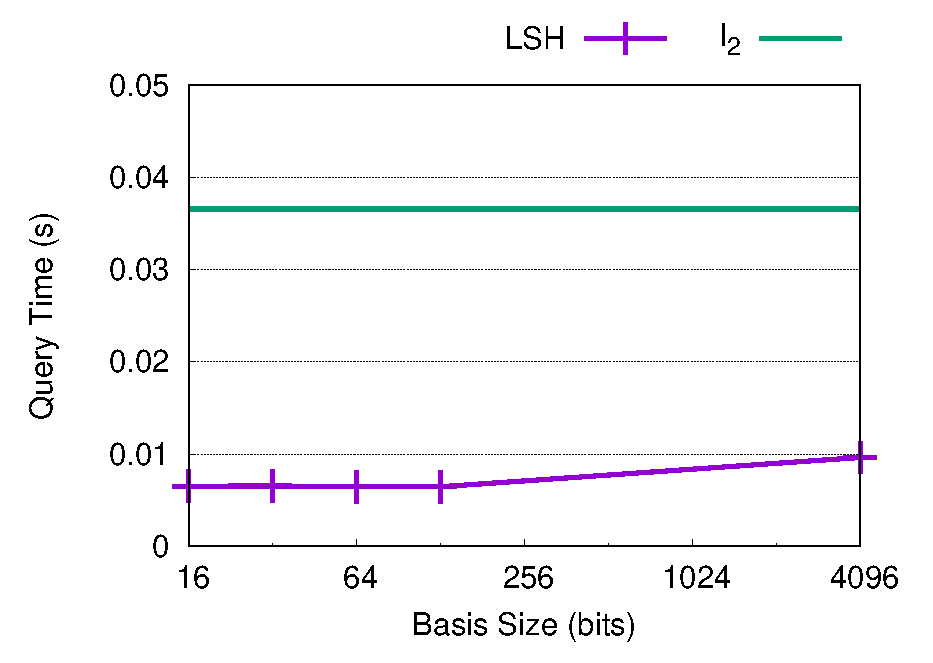
\includegraphics[width=\textwidth]{images/hashing_time_results.eps}
        \caption{Hashing query time as a function of basis size. $l_2$ speed plotted in green for comparison.}
    \end{subfigure} 
    \begin{subfigure}[t]{0.24\textwidth}
        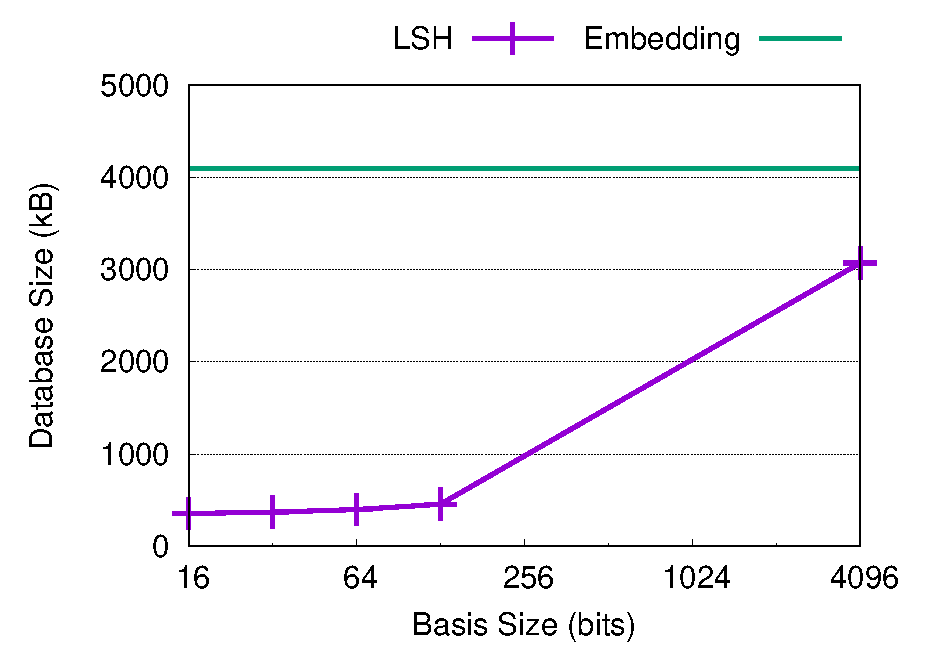
\includegraphics[width=\textwidth]{images/hashing_memory_results.eps}
        \caption{Database size as a function of basis size. Size using the embedding space plotted in green for comparison.}
    \end{subfigure}
    \caption{LSH Quantitative Results. Note that even with 4096 bits, LSH search is significantly faster and the database takes up significantly less space.}
    \label{fig:lshres}
\end{figure}

We provide an empirical study of our method using two approaches. First we test our primary task of video retrieval. This is primarily a qualitative evaluation. We show how the weights learned by our model provide a good initialization for the action recognition task with a quantitative evaluation.

\subsection{Retrieval Results}

We test several aspects of the video retrieval task. In all tests, we take the UCF101 \cite{soomro2012ucf101} training set to be our database and select a single probe video from the UCF101 test set. The videos are projected into the 128 dimensional space formed by taking the fc6 output of four six-frame stack of differences distributed uniformly at random from the video. The 128 dimensional representation for each stack of difference is averaged to give the 128 dimensional representation for each video. Our system then returns the top $n$ videos for the given probe image. We tested with $n=5$ but for brevity, only the top match is shown in the qualitative results.

Figure \ref{fig:retres} shows qualitative results of our method. Three representative probe videos were chosen for the figure that had roughly orthogonal motion types. The first video, from the "Cliff Diving" class has fast intricate motions coupled with large camera motions. The second video, from the "Bowling" class, contains constrained small motions and no camera motion. The final video, from the "Knitting" class, contains slow and highly controlled motions with the foreground occupying most of the frame. We show the top retrieval result using $l_2$ distance in the embedding space and using LSH with basis sizes of 16, 32, 64, 128, and 4096 bits. As shown in the figure, the top retrieval result correctly captures the type of motion in the probe video for $l_2$ distance. Additionally for LSH basis sizes of as small as 64 bits, the motion is still correctly captured. It is worth noting that our method does not work well on all motion types. For example, the "Knitting" class shown in the figure contains results that are qualitatively worse than the other two classes. The full retrieval results, along with videos, are provided in the supplementary material.

\begin{figure*}[t]
    \begin{center}
        \begin{tabu} to \textwidth {|X[c]|X[c]|X[c]X[c]X[c]X[c]X[c]|}
           \hline
            Probe & $l_2$ & 4096 & 128 & 64 & 32 & 16 \\ \hline \hline
            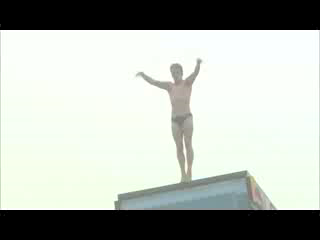
\includegraphics[width=0.1\textwidth]{images/ret_results/0/probe.png} & 
            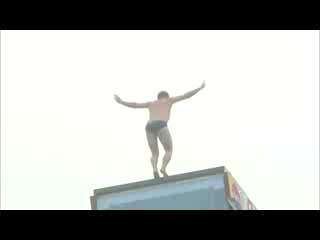
\includegraphics[width=0.1\textwidth]{images/ret_results/0/l2.png} & 
            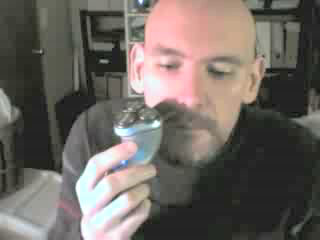
\includegraphics[width=0.1\textwidth]{images/ret_results/0/4096.png} &
            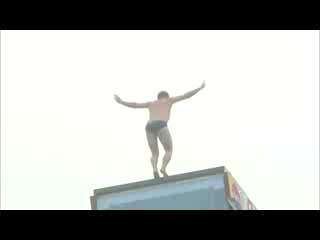
\includegraphics[width=0.1\textwidth]{images/ret_results/0/128.png} &
            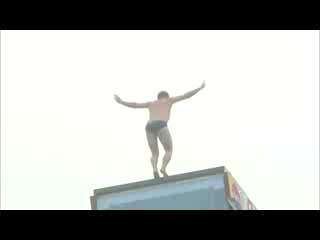
\includegraphics[width=0.1\textwidth]{images/ret_results/0/64.png} & 
            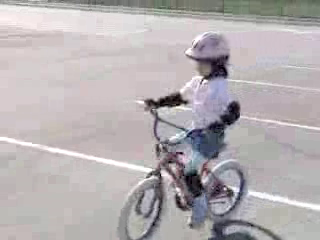
\includegraphics[width=0.1\textwidth]{images/ret_results/0/32.png} & 
            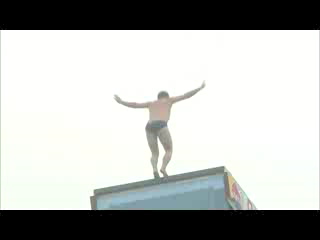
\includegraphics[width=0.1\textwidth]{images/ret_results/0/16.png} \\
            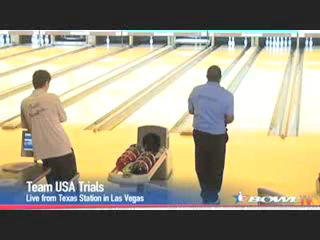
\includegraphics[width=0.1\textwidth]{images/ret_results/1/probe.png} & 
            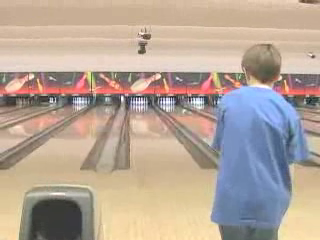
\includegraphics[width=0.1\textwidth]{images/ret_results/1/l2.png} &
            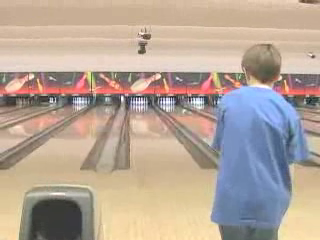
\includegraphics[width=0.1\textwidth]{images/ret_results/1/4096.png} &
            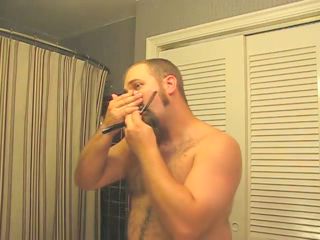
\includegraphics[width=0.1\textwidth]{images/ret_results/1/128.png} &
            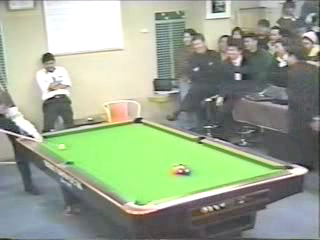
\includegraphics[width=0.1\textwidth]{images/ret_results/1/64.png} &
            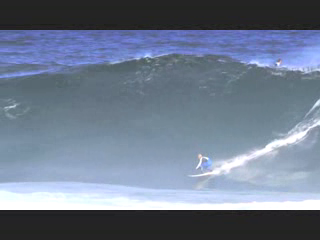
\includegraphics[width=0.1\textwidth]{images/ret_results/1/32.png} &
            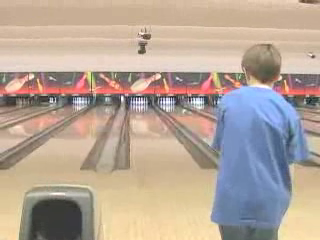
\includegraphics[width=0.1\textwidth]{images/ret_results/1/16.png} \\
            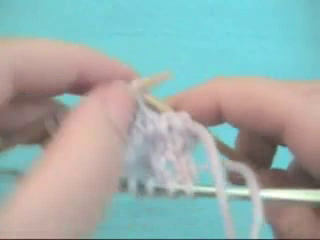
\includegraphics[width=0.1\textwidth]{images/ret_results/2/probe.png} & 
            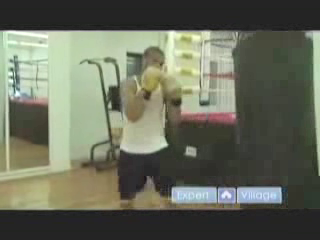
\includegraphics[width=0.1\textwidth]{images/ret_results/2/l2.png} &
            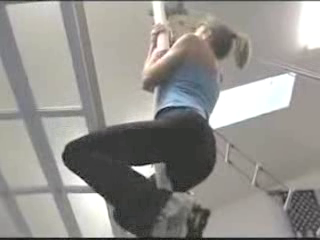
\includegraphics[width=0.1\textwidth]{images/ret_results/2/4096.png} &  
            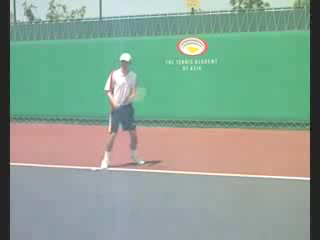
\includegraphics[width=0.1\textwidth]{images/ret_results/2/128.png} &
            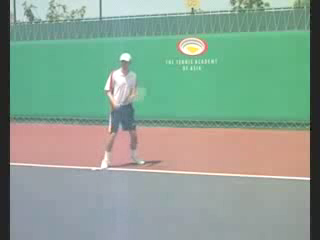
\includegraphics[width=0.1\textwidth]{images/ret_results/2/64.png} &
            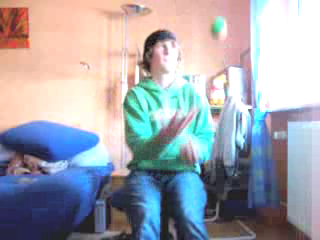
\includegraphics[width=0.1\textwidth]{images/ret_results/2/32.png} &
            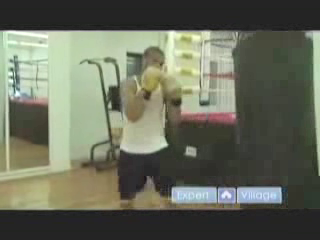
\includegraphics[width=0.1\textwidth]{images/ret_results/2/16.png} \\ \hline            
        \end{tabu}
        \caption{Qualitative retrieval results. The learned representations successfully capture similar motions in the videos. For the visualization, a single representative frame is taken from each video. The frame from the probe is shown in the left-most column. The next columns show the retrieval results for $l_2$ distance in the embedding space and for the LSH basis sizes.  }
        \label{fig:retres}
    \end{center}
\end{figure*}

Next we compare the retrieval using O3N features to ours. The results are shown in Figure \ref{fig:retcomp}. We use the same procedure to produce these results as described in the first paragraph of this section, only changing the network architecture between O3N (Section \ref{sec:o3n}) and Ours (O3N with Temporal Smoothness, Section \ref{sec:network}). The top five retrieval results are given for the same "Cliff Diving" probe that was used in Figure \ref{fig:retres}. The results show that while the O3N can capture the motion type, our method does so more effectively and can even preserve the action class. While none of the O3N results are from the "Cliff Diving" class, three out of the five are in the "Cliff Diving" class for our network. Further, the second result is from the "Still Rings" class, which contains similar acrobatic movements to the "Cliff Diving" videos. More O3N retrieval results are included in the supplementary material.

Finally, we show the quantitative effect of LSH on the system speed and memory usage in Figure \ref{fig:lshres}. For these results, the same set of LSH bases, 16, 32, 64, 128, and 4096, are used. The time to retrieve the top $n=5$ videos is computed and the total storage size of the database is reported. As the results show, LSH even with a basis size of 4096 has a significant impact on the speed of retrieval and on the size of the database. Cross referencing with Figure \ref{fig:retres}, this added efficiency comes with minimal cost in the accuracy of the retrieval results. Even at a basis size of 4096 bits, the LSH database takes up approximately one third less memory than the original database and executes queries approximately four times as quickly.

\begin{table}
    \centering
    \begin{tabu} to 0.5\textwidth {|X[l]|X[c]|}
        \hline
        Initialization & Accuracy (\%) \\ \hline \hline
        ImageNet & \textbf{66.836} \\ \hline
        O3N & 52.756 \\ \hline
        Ours (O3N + TS) & 54.072 \\ \hline
    \end{tabu}
    \caption{Fine-tuned classification accuracy for different weight initializations.}
    \label{fig:classres}
\end{table}

\subsection{Classification Accuracy Results}

We also conduct a short quantitative study by using our weights as the initialization for action recognition and fine-tuning. We follow the fine-tuning procedure in \cite{fernando2017self} for both the original O3N network and for our dual-loss architecture. The results are shown in \ref{fig:classres}, our networks weights give an improvement of around 2\% over O3N initialization.

We briefly review the fine-tuning procedure. We start with the standard AlexNet network. The convolutional layers are initialized with our weights. The fully connected layers, which now have 4096 activations, are initialized with random weights. The network is then trained for the action recognition task by using a $10^{-4}$ learning rate for the convolutional layers , which should already have reasonable weights according to our hypothesis. The fully-connected layers are trained with a $10^{-2}$ learning rate since they start with random weights. 

We tested multiple different initializations to ensure a good comparison. We follow the fine-tuning procedure described above starting from ImageNet supervised weights, O3N alone, and ours (O3N with temporal smoothness). Adding the smoothness loss gives increased accuracy over using O3N alone. As expected, the ImageNet weights perform better than both of the self-supervised weights. It is worth noting that producing ImageNet weights is very expensive: it requires a much longer training process and requires labeled data. 

\begin{figure*}[t]
    \centering
        \begin{tabu} to \textwidth {|X[c,m]|X[c,m]X[c,m]X[c,m]X[c,m]X[c,m]|}
            \hline
            Method & 0 & 1 & 2 & 3 & 4 \\ \hline \hline
            O3N & 
            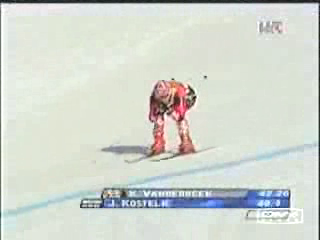
\includegraphics[width=0.1\textwidth]{images/o3vsmooth/o3/0.png}\vspace{2mm} & % vspace for presentation (otherwise images are clumpted together)
            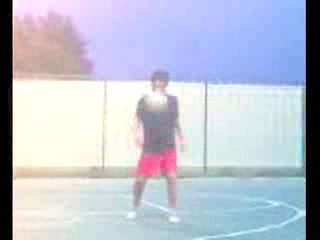
\includegraphics[width=0.1\textwidth]{images/o3vsmooth/o3/1.png}\vspace{2mm} &
            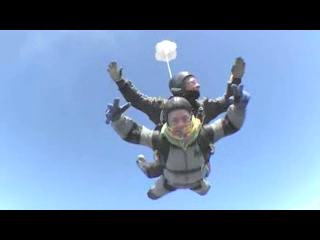
\includegraphics[width=0.1\textwidth]{images/o3vsmooth/o3/2.png}\vspace{2mm} & 
            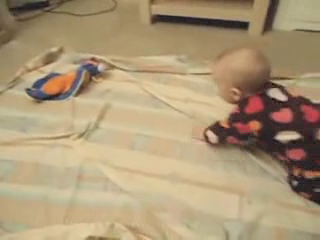
\includegraphics[width=0.1\textwidth]{images/o3vsmooth/o3/3.png}\vspace{2mm} &
            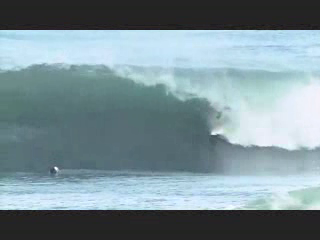
\includegraphics[width=0.1\textwidth]{images/o3vsmooth/o3/4.png}\vspace{2mm} \\
            Ours (O3N + TS) & 
            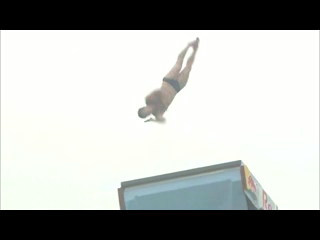
\includegraphics[width=0.1\textwidth]{images/o3vsmooth/smooth/0.png} &
            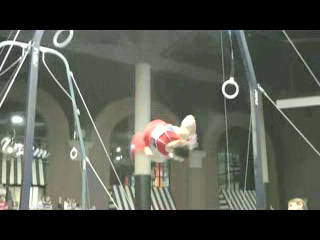
\includegraphics[width=0.1\textwidth]{images/o3vsmooth/smooth/1.png} &
            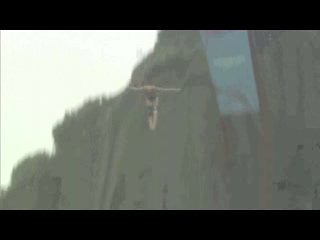
\includegraphics[width=0.1\textwidth]{images/o3vsmooth/smooth/2.png} & 
            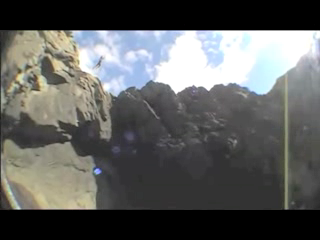
\includegraphics[width=0.1\textwidth]{images/o3vsmooth/smooth/3.png} &
            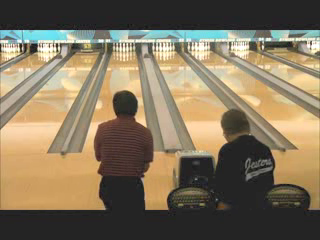
\includegraphics[width=0.1\textwidth]{images/o3vsmooth/smooth/4.png}\\ \hline            
        \end{tabu}
        \caption{Qualitative comparison, O3N vs Ours. The top five retrieval results for the same probe video for the "Cliff Diving" class in Figure \ref{fig:retres} are shown. Our method captures motion type more effectively and can preserve action class.}
        \label{fig:retcomp}
\end{figure*}



    
    \section{Conclusion and Future Work}\label{sec:conclusion}
    
	{\small
		\printbibliography
	}
	
\end{document}


